\documentclass[upLaTeX,11pt]{ujarticle}
\usepackage{amsmath,amssymb}
\usepackage{multicol}
\setlength{\topmargin}{-10mm}
\setlength{\headheight}{0mm}
\setlength{\headsep}{0mm}
\setlength{\oddsidemargin}{-10mm}
\setlength{\evensidemargin}{-10mm}
\setlength{\textwidth}{18cm}
\setlength{\textheight}{26cm}
\setlength{\columnseprule}{1mm}
%\pagestyle{empty}
\usepackage{color}
\usepackage[dvipdfmx]{graphicx}
\usepackage{multirow}
\usepackage{bigstrut}
\usepackage{url}
\usepackage[dvipdfmx]{hyperref}
\usepackage{pxjahyper}
\usepackage{here}
\hypersetup{% hyperrefオプションリスト
setpagesize=false,
 bookmarksnumbered=true,%
 bookmarksopen=true,%
 colorlinks=true,%
 linkcolor=blue,
 citecolor=red,
}
\begin{document}
\begin{center}
    {\LARGE JIA認証について}
\begin{flushright}
    増田煉瓦株式会社\\
    岩井藍 小野塚隆太 梶原豪 菊池啓亮 田島俊也 宮内礼那
\end{flushright}
\end{center}
\section{目的と背景}
増田煉瓦株式会社様にて、ピザ用ガス窯のJIA認証を取得するための諸課題の解決や製品$\cdot$工場の検査や検査方法の確立を行う。
\section{提示された課題}
\begin{itemize}
\item 燃焼部の外郭の使用する材料の詳細
\item ガス通路の気密試験
\item LPガスの消費量
\item 都市ガスの消費量
\item 電気点火性能、立ち消え安全装置
\item 工場内の設備管理
\item excelによる仕様書のテンプレートの製作
\item 内部監査
\end{itemize}
先方から提示された項目は8個あったが、解決の見通しの立ったものから取り掛かり、実現不可能だと判断したものに関しては時間の関係もあり履行すること出来なかった。
\section{解決した課題}
\subsection{ガス通路の気密試験}
気密測定は、計測に時間がかかることが問題だった。そこで、あまり漏れていないことがわかっているようなガス管の気密を60分行わずとも簡易に、安く済ませるための実験を行う。なおJIA基準では、「ガス閉止弁を通して漏れる量が70mL以下であること。ガス閉止弁を閉じた状態で、ガスの取入部に精密ガス流量計を接続し、その入口側から4.2kPaの空気圧を加えて、漏れ量を測定し、これから1時間当たりの漏れ量を算出する」となっている。

測定機器には、エスコ社のロールマノメーター(GA-7: 0~7kPa対応)を利用し、加える圧力は6kPa以上にして実験を行った。
利用した式:
\begin{equation*}
    Q=Ve\times\frac{\Delta P}{1.013\times10^5}\times\frac{60}{T}
\end{equation*}
Q:漏れ量(ml/min)、ΔP:差圧(Pa)、Ve:等価内容量(382.63 ml)、T:検出時間(s)

実験結果を次に示す。
\begin{figure}[H]
        \centering
        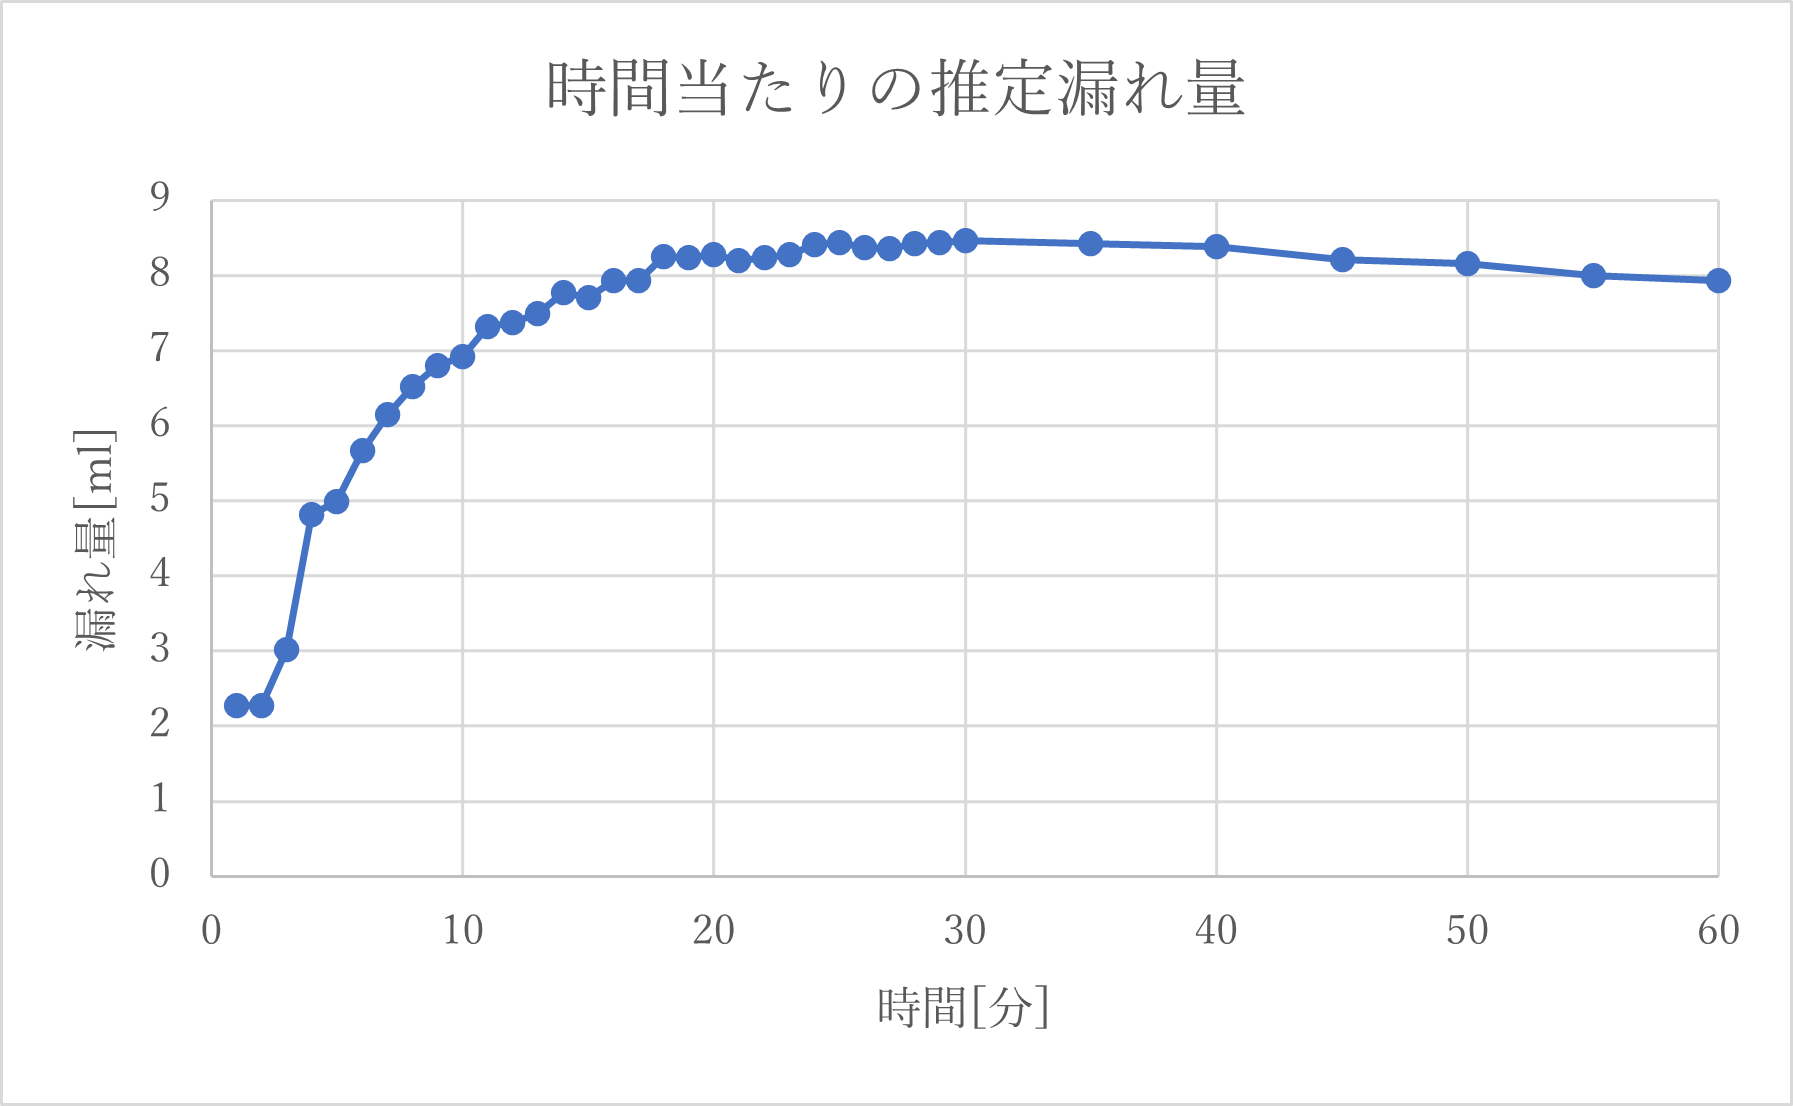
\includegraphics{画像1.png}
        \caption{漏れ量}
\end{figure}
このグラフは、その時間までの記録を基に、60分経過したときにはどの程度漏れているのかを推測した結果を表したものである。

この実験結果のグラフから、はじめの数分間は乱れているが、おおよそ10分から20分程度計測することでその結果から基準値以下であると考えることができる。
\subsection{LPガスの消費量}
JIA基準のLPガス消費量の測定では、湿式ガスメータを使用しているが、これを増田煉瓦で使用するには、校正が複雑で機器の値段が高いため、代用品としてマイコン式ガスメータとアズビル社熱式流量モニタを併用してLPガスの消費量の測定を行っている。しかし、マイコン式ガスメータとアズビル社熱式流量モニタで測定結果に10%近い差が生じている要因を把握する必要がある。表に問題解決前の両機器のガス量測定結果を示す。\\
% Table generated by Excel2LaTeX from sheet 'Sheet1'
\begin{table}[H]
    \centering
    \caption{}
      \begin{tabular}{|c|c|c|c|c|c|}
      \hline
      火力の強さ(\%) & 時間(s) & ガス量($m^3$) & マイコン($m^3/h$) & アズビル(m\^3/h) & 誤差(\%) \bigstrut\\
      \hline
      \hline
      100.0 & 111   & 0.03  & 0.97  & 0.91  & 6.19 \bigstrut[t]\\
      90.7  & 122   & 0.03  & 0.88  & 0.83  & 5.68 \\
      40.2  & 275   & 0.03  & 0.39  & 0.38  & 2.56 \bigstrut[b]\\
      \hline
      \end{tabular}%
    \label{tab:addlabel}%
  \end{table}%
  
この両機器での測定結果の誤差は各々の温度補正の設定が異なっていることが問題であることがわかった。アズビル社の熱式流量モニタの設定を変更し、再度両機器のガス量を測定した。以下に測定結果を示す。
% Table generated by Excel2LaTeX from sheet 'Sheet1'
\begin{table}[H]
    \centering
    \caption{}
      \begin{tabular}{|c|c|c|c|c|c|}
      \hline
      火力の強さ(\%) & 時間(s) & ガス量($m^3$) & マイコン($m^3/h$) & アズビル(m\^3/h) & 誤差(\%) \bigstrut\\
      \hline
      \hline
      96.9  & 114   & 0.03  & 0.94  & 0.95  & -1.06 \bigstrut[t]\\
      87.9  & 127   & 0.03  & 0.85  & 0.85  & 0.35 \\
      40.5  & 275   & 0.03  & 0.39  & 0.39  & 0.67 \bigstrut[b]\\
      \hline
      \end{tabular}%
    \label{tab:addlabel}%
  \end{table}%
  
表に示したように、設定を変更したことで、両機器の測定結果の誤差が1\%近くまで小さくなった。この様子を図で示す。
\begin{figure}[H]
    \centering
    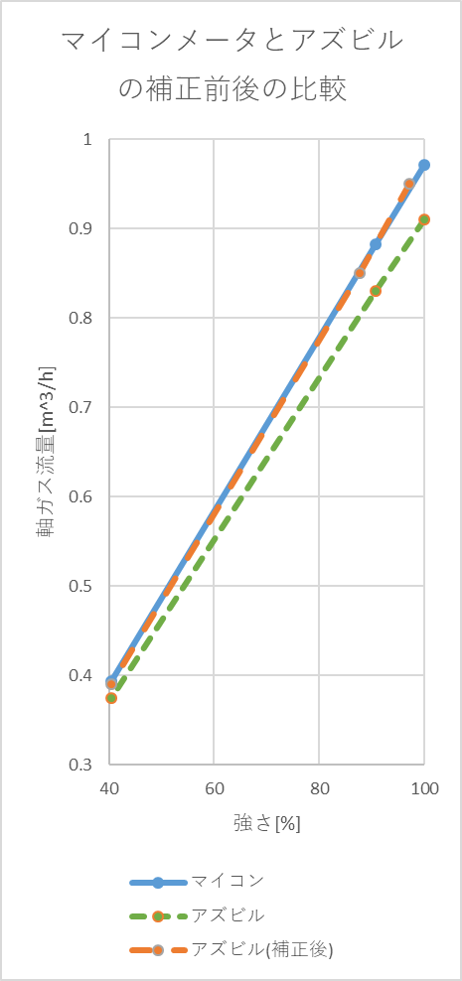
\includegraphics{result3.png}
    \caption{}
\end{figure} 

マイコン式ガスメータとアズビル社熱式流量モニタでの測定値の違いは、温度補正が主なものであることが分かった。しかし、他の要因として、ガス配管系統内での気密性、各々のそもそもの仕組みの違いもあると考えられる。
\subsection{燃焼状態試験}
JIA認証では燃焼状態を評価するために、以下の項目について検査を行った。
\begin{itemize}
    \item 火移り\\
    確実に火移りし、爆発的に着火しないこと
    \item リフティング\\
    リフティングがないこと
    \item 消火\\
    消火がないこと
    \item 炎の均一性\\
    炎が均一であること
    \item 逆火\\
    逆火がないこと
    \item 消火音\\
    爆発音のないこと
    \item すすの発生\\
    すすの発生がないこと
    \item 黄炎の接触\\
    電極部に常時接触しないこと
    \item パイロットバーナの炎の安定性\\
    消火又は逆火のないこと
\end{itemize}
すべての検査項目において、検査基準を満たしていることが確認できた。
\subsection{電気点火性能}
JIA認証では電気点火性能を評価する必要がある。電気点火性能の試験方法は、10回繰り返して点火操作を行い、点火回数(9回以上点火する)、ケーシング外への炎のあふれ及び爆発的に点火(騒音が85dB以下)しないことを確認することである。また、検査細則で、ガス量は、最大及び最小の状態についても確認することと、試験ガスは、不完全燃焼しやすいガスと、吹き消えしやすいガスを使用することとされている。しかし、増田煉瓦株式会社様では試験ガスがないため、条件を厳しくするためにスパーク距離を点火しなくなる間際の長さにして試験を行った。電源の最大電圧はスライダックで設定出来る最大の120.7V、最小電圧は点火できる最小電圧であった72Vとした。以下に検査結果を示す。
\begin{table}[H]
    \centering
    \caption{電源電圧(72V)}
    \begin{tabular}{|l|l|l|l|l|l|l|l|l|l|l|}
    \hline
      & 1 & 2 & 3 & 4 & 5 & 6 & 7 & 8 & 9 & 10 \\ \hline
    弱 & 〇 & 〇 & 〇 & 〇 & 〇 & 〇 & 〇 & 〇 & 〇 & 〇  \\ \hline
    強 & 〇 & 〇 & 〇 & 〇 & 〇 & 〇 & 〇 & 〇 & 〇 & 〇  \\ \hline
    \end{tabular}
\end{table}

\begin{table}[H]
    \centering
    \caption{電源電圧(120.7V)}
    \begin{tabular}{|l|l|l|l|l|l|l|l|l|l|l|}
        \hline
          & 1 & 2 & 3 & 4 & 5 & 6 & 7 & 8 & 9 & 10 \\ \hline
          弱 & 〇 & 〇 & 〇 & 〇 & 〇 & 〇 & 〇 & 〇 & 〇 & 〇  \\ \hline
          強 & 〇 & 〇 & 〇 & 〇 & 〇 & 〇 & 〇 & 〇 & 〇 & 〇  \\ \hline
    \end{tabular}
\end{table}

\begin{table}[H]
    \centering
    \caption{スパーク距離(5mm)}
    \begin{tabular}{|l|l|l|l|l|l|l|l|l|l|l|}
        \hline
          & 1 & 2 & 3 & 4 & 5 & 6 & 7 & 8 & 9 & 10 \\ \hline
          弱 & 〇 & 〇 & 〇 & 〇 & 〇 & 〇 & 〇 & 〇 & 〇 & 〇  \\ \hline
          強 & 〇 & 〇 & 〇 & 〇 & 〇 & 〇 & 〇 & 〇 & 〇 & 〇  \\ \hline
    \end{tabular}
\end{table}

\begin{table}[H]
    \centering
    \caption{スパーク距離(3mm)}
    \begin{tabular}{|l|l|l|l|l|l|l|l|l|l|l|}
        \hline
          & 1 & 2 & 3 & 4 & 5 & 6 & 7 & 8 & 9 & 10 \\ \hline
          弱 & 〇 & 〇 & 〇 & 〇 & 〇 & 〇 & 〇 & 〇 & 〇 & 〇  \\ \hline
          強 & 〇 & 〇 & 〇 & 〇 & 〇 & 〇 & 〇 & 〇 & 〇 & 〇  \\ \hline
    \end{tabular}
\end{table}

以上の表で示したように、試験を行ったすべての条件で点火することが確認できた。
\subsection{excelによる仕様書のテンプレートの製作}
\subsection{内部監査}
お互いの実験内容について各班で確認、不備や不明瞭な点を指摘し、担当した班が回答書を作成することを行った。以下に行ったときの内容を表に示す。
  
\section{まとめ}
\section{謝辞}
本実験を進めるにあたり多大なご指導をいただいた増田煉瓦株式会社の技術担当中島様をはじめ、多くの関係者の皆様に深く感謝申し上げます。
\end{document}